\documentclass{article} % Document class
\usepackage[a3paper, total={6in, 10in}]{geometry}
\usepackage{graphicx}
\usepackage{xcolor}
\title{Your Paper}
\author{sameena Begum}
\date{\today}
\begin{document}
\maketitle
Your abstract\section{Introduction}
Youur introduction goes here! Simply start writing your document and use the Recompile button to
view the updated PDF preview. Examples of commonly used commands and features are listed below,
to help you get started.
Once you’re familiar with the editor, you can find various project setting in the Overleaf menu,
accessed via the button in the very top left of the editor. To view tutorials, user guides, and further
documentation, please visit our \textcolor{blue}{help library}, or head to our plans page to \textcolor{blue}{choose your plan}.
\subsection{ Some examples to get started}
\subsection{How to create Sections and Subsections}
Simply use the section and subsection commands, as in this example document! With Overleaf, all
the formatting and numbering is handled automatically according to the template you’ve chosen. If
you’re using Rich Text mode, you can also create new section and subsections via the buttons in the editor toolbar.
\subsection{How to include Figures}
First you have to upload the image file from your computer using the upload link in the file-tree menu.
Then use the includegraphics command to include it in your document. Use the figure environment
and the caption command to add a number and a caption to your figure. See the code for Figure 1 in this section for an example.
Note that your figure will automatically be placed in the most appropriate place for it, given the surrounding text and taking into account other figures or tables that may be close by. You can find
out more about adding images to your documents in this help article on \textcolor{blue}{including images on Overleaf}.
\begin{figure}
		\centering
		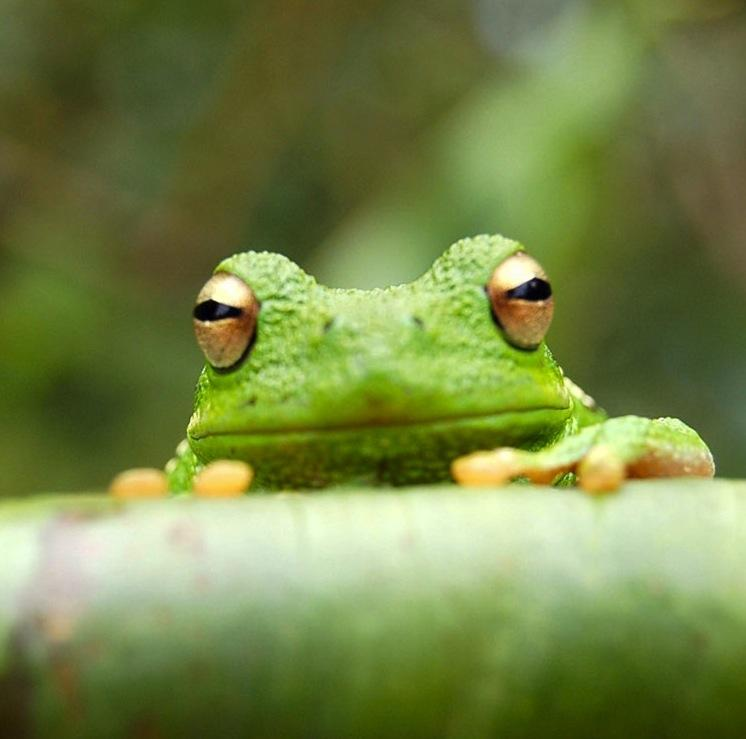
\includegraphics[width=0.4\textwidth]{frog.jpg}
		\caption{his frog was uploaded via the file-tree menu.}
		\label{fig:example}
	\end{figure}
\begin{table}[h]
	\centering
	\begin{tabular}{|c|c|}
	\textbf{item} & \textbf{Quality} \\
		\hline
		widgets &42\\
		gagets &13\\
	\end{tabular}
	\caption{Example Table}
	\label{tab:example}
\subsection{How to add Tables}
Use the table and tabular environments for basic tables — see Table 1, for example. For more infor-
	mation, please see this help article \textcolor{blue}{on tables}.
\subsection{how to add Comments and tracks changes}
Comments can be added to your project by highlighting some text and clicking “Add comment” in
the top right of the editor pane. To view existing comments, click on the Review menu in the toolbar
above. To reply to a comment, click on the Reply button in the lower right corner of the comment.
You can close the Review pane by clicking its name on the toolbar when you’re done reviewing for the
time being.
Track changes are available on all our\textcolor{blue} {premium plans}, and can be toggled on or off using the option
at the top of the Review pane. Track changes allow you to keep track of every change made to the
document, along with the person making the change.
\subsection{How to add Lists}
	You can make lists with automatic numbering .
	\subsection{Lists}
	\begin{enumerate} 
		\item like this.
		\item and like this...
		
		....or bullet point...
		\end{enumerate}
		\begin{itemize}
		
		\item like this...
		\item and like this....
	\end{itemize}
\subsubsection{How to write Mathematics}
	L A TEX is great at typesetting mathematics. Let X 1 , X 2 , . . . , X n be a sequence of independent and dentically distributed random variables with E[$\mu$] =$\mu$ and Var[$X_i$]
=$\sigma^2$\textless$\infty$. and let \[S_n=\frac{X_1+ X_2+....+X_n}{n}=\frac{1}{n}\sum-{i}^{n} X_i\]

denote their mean. Then as n approach infinity
\subsection{How to change the margins and paper size}
	Usually the template you’re using will have the page margins and paper size set correctly for that
	use-case. For example, if you’re using a journal article template provided by the journal publisher,
	that template will be formatted according to their requirements. In these cases, it’s best not to alter
	the margins directly.
	If however you’re using a more general template, such as this one, and would like to alter the
	margins, a common way to do so is via the geometry package. You can find the geometry package
	loaded in the preamble at the top of this example file, and if you’d like to learn more about how to
	adjust the settings, please visit this help article on \textcolor{blue}{page size and margins}.
	\subsection{How to change the document language and spell check settings}
		Overleaf supports many different languages, including multiple different languages within one docu-
		ment.
		To configure the document language, simply edit the option provided to the babel package in the
		preamble at the top of this example project. To learn more about the different options, please visit
		this help article on \textcolor{blue}{international language} support.
		To change the spell check language, simply open the Overleaf menu at the top left of the editor
		window, scroll down to the spell check setting, and adjust accordingly.
		\subsection{How to add Citations and a References List}
			You can simply upload a .bib file containing your BibTeX entries, created with a tool such as JabRef.
			You can then cite entries from it, like this: \textcolor{blue}{[Gre93]}. Just remember to specify a bibliography style, as
			well as the filename of the .bib. You can find a \textcolor{blue}{video tutorial} here to learn more about BibTeX.
			If you have an \textcolor{blue}{upgraded account}, you can also import your Mendeley or Zotero library directly as
			a .bib file, via the upload menu in the file-tree.
			\subsection{Good luck!}
				We hope you find Overleaf useful, and do take a look at our\textcolor{blue}{help library}for more tutorials and user
				guides! Please also let us know if you have any feedback using the Contact Us link at the bottom of
				the Overleaf menu — or use the contact form at\textcolor{blue} {https://www.overleaf.com/contact.}
				\section{References}
					[Gre93] George D. Greenwade.
					14(3):342–351, 1993.
					The Comprehensive Tex Archive Network (CTAN).
					3
					TUGBoat,
				
		\end{table}
\end{document}
